%%%%%%%%%%%%%%%%%%%%%%%%%%%%%%%%%%%%%%%%%%%%%%%%%%%%%%%%%%%%%%%%%%%%%%%%%%%%%
%
%  System        : 
%  Module        : 
%  Object Name   : $RCSfile$
%  Revision      : $Revision$
%  Date          : $Date$
%  Author        : $Author$
%  Created By    : Robert Heller
%  Created       : Fri May 3 11:25:06 2024
%  Last Modified : <240503.2153>
%
%  Description 
%
%  Notes
%
%  History
% 
%%%%%%%%%%%%%%%%%%%%%%%%%%%%%%%%%%%%%%%%%%%%%%%%%%%%%%%%%%%%%%%%%%%%%%%%%%%%%
%
%    Copyright (C) 2024  Robert Heller D/B/A Deepwoods Software
%			51 Locke Hill Road
%			Wendell, MA 01379-9728
%
%    This program is free software; you can redistribute it and/or modify
%    it under the terms of the GNU General Public License as published by
%    the Free Software Foundation; either version 2 of the License, or
%    (at your option) any later version.
%
%    This program is distributed in the hope that it will be useful,
%    but WITHOUT ANY WARRANTY; without even the implied warranty of
%    MERCHANTABILITY or FITNESS FOR A PARTICULAR PURPOSE.  See the
%    GNU General Public License for more details.
%
%    You should have received a copy of the GNU General Public License
%    along with this program; if not, write to the Free Software
%    Foundation, Inc., 675 Mass Ave, Cambridge, MA 02139, USA.
%
% 
%
%%%%%%%%%%%%%%%%%%%%%%%%%%%%%%%%%%%%%%%%%%%%%%%%%%%%%%%%%%%%%%%%%%%%%%%%%%%%%

\documentclass[12pt,twoside,letterpaper]{article}
\usepackage{graphicx}
\usepackage{mathptm}
\usepackage{times}
\usepackage{makeidx}
\usepackage{ifpdf}
\usepackage{footmisc}
\ifpdf
\usepackage[pdftex,
            pagebackref=true,
            colorlinks=true,
            linkcolor=blue,
            unicode
           ]{hyperref}
\else
\usepackage[ps2pdf,
            pagebackref=true,
            colorlinks=true,
            linkcolor=blue,
            unicode
           ]{hyperref}
\usepackage{pspicture}
\fi
\usepackage{url}
\pagestyle{headings}
\emergencystretch=50pt
\setcounter{tocdepth}{3}
\setcounter{secnumdepth}{3}
\title{FRED (EOT) flashing board.}
\author{Robert Heller \\ The Country Robot \\ Wendell, MA, USA}
\date{\today}
\begin{document}
\maketitle

This is a circuit board that implements a FRED (Flashing Rear End 
Device)\footnote{Also know as an EOT (End Of Train) device.}. This little 
circuit board rides in the trailing truck of the last freight car of a train 
and flashes a LED mounted on a FRED riding in the trailing coupler of that 
freight car.

\section{Assembly}

\begin{figure}[hbpt]\begin{centering}%
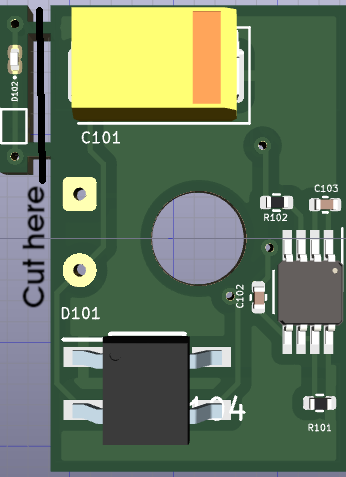
\includegraphics[width=3in]{FRED_Board3D_Top_cut.png}
\caption{Cutting the boards apart}
\label{fig:boardcut}
\end{centering}\end{figure}
The circuit board is mostly assembled.  It is necessary to solder on two small 
pieces of phosphor bronze that will be the wiper contacts to pick up power 
from the track. The two small pieces of phosphor bronze are soldered onto the 
labeled pad on the back side of the board and then bent into ``V'' shapes. It 
is also necessary to cut the board into two pieces, as shown in 
Figure~\ref{fig:boardcut}. After cutting the boards apart, carefully sand the 
cuts flush.

\begin{figure}[hbpt]\begin{centering}%
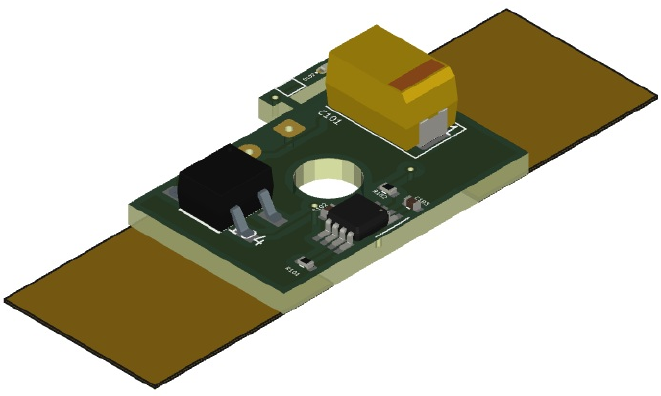
\includegraphics[width=3in]{FRED_with_wipers_not_bent.png}
\caption{Wiper strips soldered on}
\label{fig:FRED_with_wipers_not_bent}
\end{centering}\end{figure}
Next cut two pieces of phosphor bronze sheet, 13.5mm x 16mm and solder them to
the pads on the bottom at the ends of the nain board, with 12.5mm extending
beyond the ends of the board, as shown in
Figure~\ref{fig:FRED_with_wipers_not_bent}. Once soldered, bend the pieces up
(under the board) as shown in the photo in Figure~\ref{fig:wiperphoto}.











\end{document}
